\documentclass[tikz,border=1.5pt]{standalone}

\usepackage{amsmath}
\usepackage{xcolor}
\usepackage{helvet}
\renewcommand{\familydefault}{\sfdefault}

\usetikzlibrary{arrows.meta,calc}

\definecolor{slate}{HTML}{46515E}
\definecolor{inputfill}{HTML}{F3F4F6}
\definecolor{encoderfill}{HTML}{E6EBF3}
\definecolor{guardfill}{HTML}{B9D2E7}
\definecolor{outputfill}{HTML}{F1F0EB}
\definecolor{whitebox}{HTML}{FBFCFE}
\definecolor{fusionfill}{HTML}{EEF3F8}
\definecolor{modelfill}{HTML}{EAF2FB}
\definecolor{stagefill}{HTML}{DDECFF}
\definecolor{guardstroke}{HTML}{2F638F}
\definecolor{knownfill}{HTML}{DCEFD7}
\definecolor{knownstroke}{HTML}{3F7A46}
\definecolor{unkfill}{HTML}{F9DEDA}
\definecolor{unkstroke}{HTML}{B23A3A}
\definecolor{attackfill}{HTML}{EEE2F4}
\definecolor{attackstroke}{HTML}{7A5C84}
\definecolor{llmfill}{HTML}{EEEEEE}
\definecolor{qrcwosfill}{HTML}{DCEFE5}
\definecolor{qrcwosstroke}{HTML}{5A7868}

\begin{document}

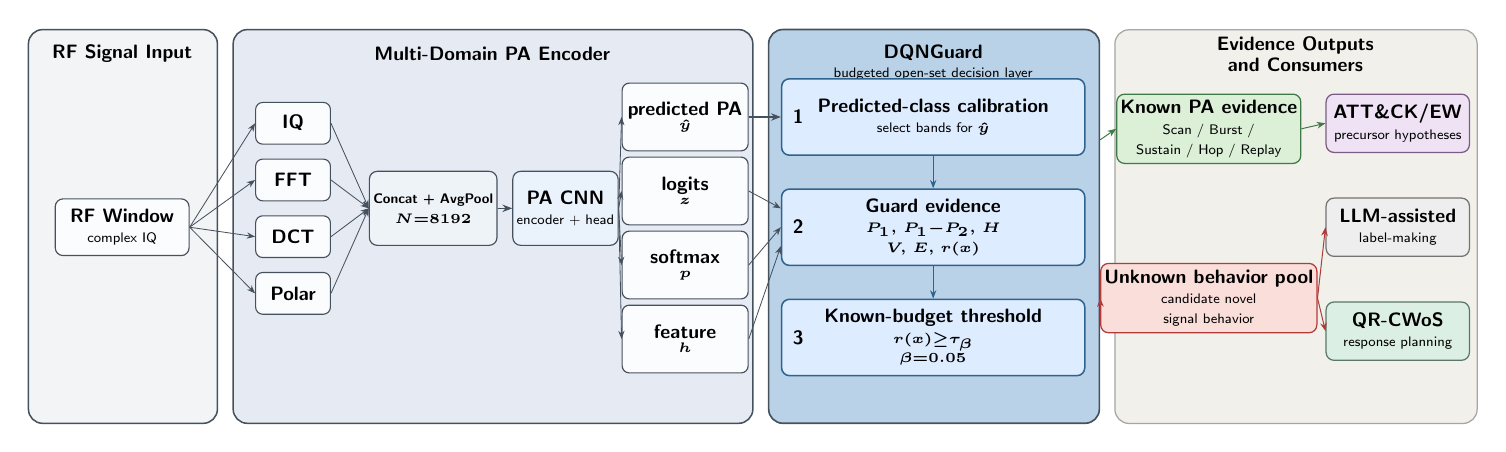
\begin{tikzpicture}[
  x=1mm,
  y=1mm,
  font=\sffamily,
  inputpanel/.style={
    draw=slate,
    fill=inputfill,
    rounded corners=1.8mm,
    line width=0.55pt,
    inner sep=0pt
  },
  encoderpanel/.style={
    draw=slate,
    fill=encoderfill,
    rounded corners=1.8mm,
    line width=0.55pt,
    inner sep=0pt
  },
  guardpanelstyle/.style={
    draw=slate,
    fill=guardfill,
    rounded corners=1.8mm,
    line width=0.60pt,
    inner sep=0pt
  },
  outputpanelstyle/.style={
    draw=black!35,
    fill=outputfill,
    rounded corners=1.8mm,
    line width=0.45pt,
    inner sep=0pt
  },
  block/.style={
    draw=slate,
    fill=whitebox,
    rounded corners=1.0mm,
    line width=0.42pt,
    align=center,
    inner sep=1.4pt,
    font=\sffamily\scriptsize
  },
  smallblock/.style={
    draw=slate,
    fill=whitebox,
    rounded corners=0.9mm,
    line width=0.40pt,
    align=center,
    inner sep=1.2pt,
    font=\sffamily\bfseries\scriptsize
  },
  metric/.style={
    draw=slate,
    fill=whitebox,
    rounded corners=0.9mm,
    line width=0.42pt,
    align=center,
    inner sep=1.4pt,
    font=\sffamily\bfseries\tiny
  },
  stage/.style={
    draw=guardstroke,
    fill=stagefill,
    rounded corners=1.0mm,
    line width=0.55pt,
    align=center,
    inner sep=1.5pt,
    font=\sffamily\scriptsize
  },
  knownbox/.style={
    draw=knownstroke,
    fill=knownfill,
    rounded corners=1.0mm,
    line width=0.45pt,
    align=center,
    inner sep=1.3pt,
    font=\sffamily\scriptsize
  },
  unknownbox/.style={
    draw=unkstroke,
    fill=unkfill,
    rounded corners=1.0mm,
    line width=0.45pt,
    align=center,
    inner sep=1.3pt,
    font=\sffamily\scriptsize
  },
  attackbox/.style={
    draw=attackstroke,
    fill=attackfill,
    rounded corners=1.0mm,
    line width=0.45pt,
    align=center,
    inner sep=1.3pt,
    font=\sffamily\scriptsize
  },
  llmbox/.style={
    draw=black!55,
    fill=llmfill,
    rounded corners=1.0mm,
    line width=0.45pt,
    align=center,
    inner sep=1.3pt,
    font=\sffamily\scriptsize
  },
  qrcwosbox/.style={
    draw=qrcwosstroke,
    fill=qrcwosfill,
    rounded corners=1.0mm,
    line width=0.45pt,
    align=center,
    inner sep=1.3pt,
    font=\sffamily\scriptsize
  },
  arr/.style={
    -{Stealth[length=1.25mm,width=0.95mm]},
    draw=slate,
    line width=0.38pt,
    shorten >=0pt,
    shorten <=0pt
  },
  thinarr/.style={
    -{Stealth[length=1.05mm,width=0.80mm]},
    draw=slate,
    line width=0.30pt,
    shorten >=0pt,
    shorten <=0pt
  },
  knownarr/.style={
    -{Stealth[length=1.10mm,width=0.85mm]},
    draw=knownstroke,
    line width=0.36pt,
    shorten >=0pt,
    shorten <=0pt
  },
  unkarr/.style={
    -{Stealth[length=1.10mm,width=0.85mm]},
    draw=unkstroke,
    line width=0.36pt,
    shorten >=0pt,
    shorten <=0pt
  }
]

% ---------------------------------------------------------------------
% Panels
% ---------------------------------------------------------------------
\node[inputpanel, minimum width=24mm, minimum height=50mm, anchor=south west] (inputpanel) at (0,0) {};
\node[encoderpanel, minimum width=66mm, minimum height=50mm, anchor=south west] (encpanel) at (26,0) {};
\node[guardpanelstyle, minimum width=42mm, minimum height=50mm, anchor=south west] (guardpanel) at (94,0) {};
\node[outputpanelstyle, minimum width=46mm, minimum height=50mm, anchor=south west] (outpanel) at (138,0) {};

% Panel titles
\node[font=\sffamily\bfseries\scriptsize] at (12,47.0) {RF Signal Input};
\node[font=\sffamily\bfseries\scriptsize] at (59,47.0) {Multi-Domain PA Encoder};
\node[font=\sffamily\bfseries\scriptsize] at (115,47.2) {DQNGuard};
\node[font=\sffamily\tiny] at (115,44.5) {budgeted open-set decision layer};
\node[font=\sffamily\bfseries\scriptsize, align=center] at (161,47.0) {Evidence Outputs\\[-0.5pt] and Consumers};

% ---------------------------------------------------------------------
% RF input
% ---------------------------------------------------------------------
\node[block, minimum width=17mm, minimum height=7.2mm] (rf) at (12,25.0)
{\textbf{RF Window}\\[-0.6pt] {\tiny complex IQ}};

% ---------------------------------------------------------------------
% Transform stack
% ---------------------------------------------------------------------
\node[smallblock, minimum width=9.5mm, minimum height=5.3mm] (iq)    at (33.7,38.2) {IQ};
\node[smallblock, minimum width=9.5mm, minimum height=5.3mm] (fft)   at (33.7,31.0) {FFT};
\node[smallblock, minimum width=9.5mm, minimum height=5.3mm] (dct)   at (33.7,23.8) {DCT};
\node[smallblock, minimum width=9.5mm, minimum height=5.3mm] (polar) at (33.7,16.6) {Polar};

% Fusion and model
\node[block, fill=fusionfill, minimum width=15.5mm, minimum height=9.4mm] (fusion) at (51.5,27.4)
{\textbf{\tiny Concat + AvgPool}\\[-0.8pt] $\boldsymbol{\scriptstyle N=8192}$};

\node[block, fill=modelfill, minimum width=12.8mm, minimum height=9.4mm] (cnn) at (68.3,27.4)
{\textbf{\scriptsize PA CNN}\\[-0.8pt] {\tiny encoder + head}};

% Metrics, ordered for clean routing
\node[metric, minimum width=16.0mm, minimum height=8.6mm] (yhat) at (83.5,39.0)
{\textbf{\scriptsize predicted PA}\\[-1pt] $\boldsymbol{\hat{y}}$};

\node[metric, minimum width=16.0mm, minimum height=8.6mm] (zlog) at (83.5,29.6)
{\textbf{\scriptsize logits}\\[-1pt] $\boldsymbol{z}$};

\node[metric, minimum width=16.0mm, minimum height=8.6mm] (psoft) at (83.5,20.2)
{\textbf{\scriptsize softmax}\\[-1pt] $\boldsymbol{p}$};

\node[metric, minimum width=16.0mm, minimum height=8.6mm] (hfeat) at (83.5,10.8)
{\textbf{\scriptsize feature}\\[-1pt] $\boldsymbol{h}$};

% ---------------------------------------------------------------------
% DQNGuard stages
% ---------------------------------------------------------------------
\node[stage, minimum width=38.5mm, minimum height=9.7mm] (cal) at (115,39.0)
{\textbf{\scriptsize Predicted-class calibration}\\[-0.6pt] {\tiny select bands for $\boldsymbol{\hat{y}}$}};

\node[stage, minimum width=38.5mm, minimum height=9.7mm] (evid) at (115,25.0)
{\textbf{\scriptsize Guard evidence}\\[-0.6pt]
$\boldsymbol{\scriptstyle P_1,\;P_1-P_2,\;H}$\\[-1.0pt]
$\boldsymbol{\scriptstyle V,\;E,\;r(x)}$};

\node[stage, minimum width=38.5mm, minimum height=9.7mm] (thresh) at (115,11.0)
{\textbf{\scriptsize Known-budget threshold}\\[-0.6pt]
$\boldsymbol{\scriptstyle r(x)\ge \tau_\beta}$\\[-1.0pt]
$\boldsymbol{\scriptstyle \beta=0.05}$};

\node[font=\sffamily\bfseries\scriptsize] at ($(cal.west)+(2.2,0)$) {1};
\node[font=\sffamily\bfseries\scriptsize] at ($(evid.west)+(2.2,0)$) {2};
\node[font=\sffamily\bfseries\scriptsize] at ($(thresh.west)+(2.2,0)$) {3};

% ---------------------------------------------------------------------
% Outputs
% ---------------------------------------------------------------------
\node[knownbox, minimum width=20.5mm, minimum height=8.8mm] (known) at (150.0,37.5)
{\textbf{\scriptsize Known PA evidence}\\[-0.6pt]
{\tiny Scan / Burst /}\\[-0.8pt]
{\tiny Sustain / Hop / Replay}};

\node[unknownbox, minimum width=22.4mm, minimum height=8.8mm] (unknown) at (150.0,16.0)
{\textbf{\scriptsize Unknown behavior pool}\\[-0.6pt]
{\tiny candidate novel}\\[-0.8pt]
{\tiny signal behavior}};

\node[attackbox, minimum width=18.2mm, minimum height=7.4mm] (attack) at (174.0,38.2)
{\textbf{\scriptsize ATT\&CK/EW}\\[-0.6pt] {\tiny precursor hypotheses}};

\node[llmbox, minimum width=18.2mm, minimum height=7.4mm] (llm) at (174.0,25.0)
{\textbf{\scriptsize LLM-assisted}\\[-0.6pt] {\tiny label-making}};

\node[qrcwosbox, minimum width=18.2mm, minimum height=7.4mm] (qrcwos) at (174.0,11.8)
{\textbf{\scriptsize QR-CWoS}\\[-0.6pt] {\tiny response planning}};

% ---------------------------------------------------------------------
% Arrows
% ---------------------------------------------------------------------
\draw[thinarr] (rf.east) -- (iq.west);
\draw[thinarr] (rf.east) -- (fft.west);
\draw[thinarr] (rf.east) -- (dct.west);
\draw[thinarr] (rf.east) -- (polar.west);

\draw[thinarr] (iq.east) -- (fusion.west);
\draw[thinarr] (fft.east) -- (fusion.west);
\draw[thinarr] (dct.east) -- (fusion.west);
\draw[thinarr] (polar.east) -- (fusion.west);

\draw[arr] (fusion.east) -- (cnn.west);

\draw[thinarr] (cnn.east) -- (yhat.west);
\draw[thinarr] (cnn.east) -- (zlog.west);
\draw[thinarr] (cnn.east) -- (psoft.west);
\draw[thinarr] (cnn.east) -- (hfeat.west);

\draw[arr] (yhat.east) -- (cal.west);
\draw[thinarr] (zlog.east) -- ($(evid.west)+(0,2.4)$);
\draw[thinarr] (psoft.east) -- (evid.west);
\draw[thinarr] (hfeat.east) -- ($(evid.west)+(0,-2.4)$);

\draw[thinarr, draw=guardstroke] (cal.south) -- (evid.north);
\draw[thinarr, draw=guardstroke] (evid.south) -- (thresh.north);

\draw[knownarr] ($(guardpanel.east)+(0,11.0)$) -- (known.west);
\draw[unkarr] ($(guardpanel.east)+(0,-9.5)$) -- (unknown.west);

\draw[knownarr] (known.east) -- (attack.west);
\draw[unkarr] (unknown.east) -- (llm.west);
\draw[unkarr] (unknown.east) -- (qrcwos.west);

\end{tikzpicture}

\end{document}
